\chapter{El principio de \emph{D'Alembert}}



	
\begin{tikzpicture}
	\fill [left color=red!50, right color=teal!50] (0,0) rectangle (6.5,.1);
	\fill [left color=teal!50, right color=blue!50] (6.5,0) rectangle (11.5,.1);
	\end{tikzpicture}

\vspace{1cm}

\begin{adjustwidth}{50pt}{50pt}
\begin{ejemplo}
	En este tema veremos otro modo de resolver un sencillo problema de estática distinto a como se resuelve en mecánica newtoniana, usaremos el \emph{principio de D'Alembert}.	
\end{ejemplo}
\end{adjustwidth}
	
\vspace{1cm}
	
\section{Principio de \emph{D'Alembert} o de los Trabajos Virtuales}\label{T1PTV}

\vspace{0.5cm}

\begin{myblock}{Principio de D'Alembert para el caso estático}
$\,$

\begin{Large}
\begin{equation}
\label{DA}
 \displaystyle \sum_i \ \overrightarrow{F_i}^{(a)} \cdot \delta \overrightarrow{r_i}	 \ = \ 0
\end{equation}
\end{Large}
$\,$
\end{myblock}

\vspace{1cm}
\normalsize{Pronto} veremos el significado de esta ecuación. Empecemos analizando un sencillo ejemplo por dos métodos distintos: usando la conocida \emph{mecánica newtoniana} (ejemplo 1) y aplicando el \emph{Principio de D'Alembert o de los Trabajos Virtuales} (ejemplo 2).

\vspace{1cm}

\begin{example}
.	Determinar la \emph{fuerza de fricción} $F$ para que la barra rígida, uniforme y homogénea de masa $M$ y longitud $L$, apoyada en una esquina recta con ángulo $\theta$ se encuentre en equilibrio, \textbf{\emph{caso estático}}.

	\begin{figure}[H]
		\centering
		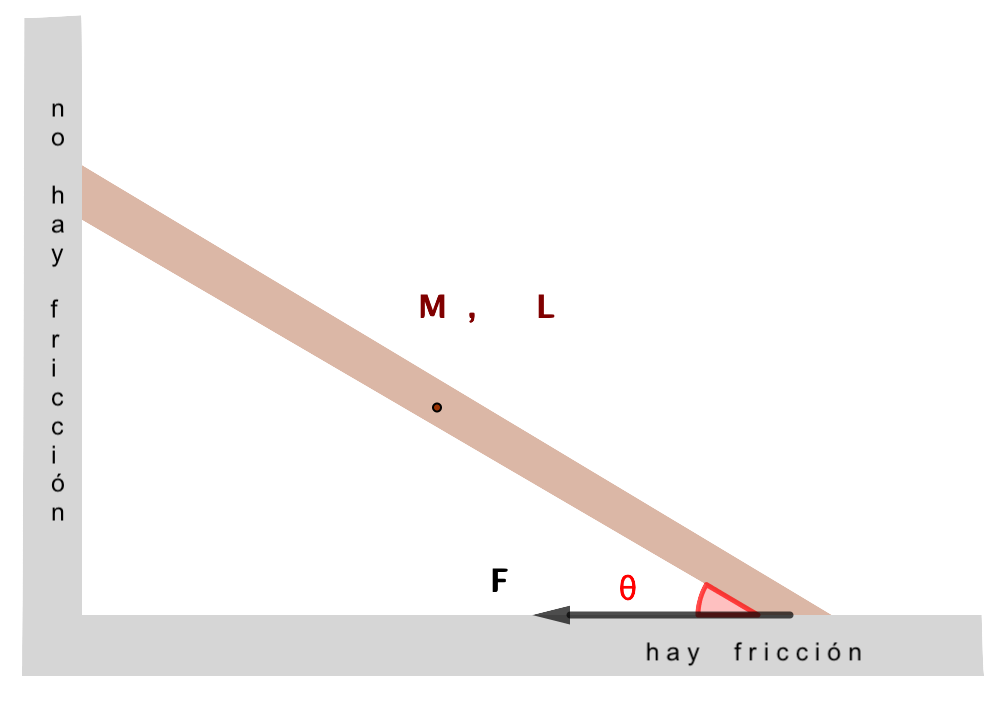
\includegraphics[width=.6\textwidth]{imagenes/img01-01.png}
	\end{figure}
	
	\begin{small}
	\textcolor{gris}{Hemos dibujado la fuerza de fricción, $F$, hacia la izquierda,  significando que se opone al movimiento.}	
	\end{small}

\end{example}

\vspace{1cm}
\subsection{Resolución por mecánica newtoniana}
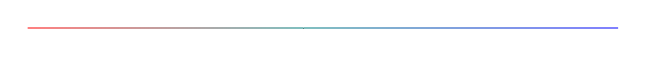
\begin{tikzpicture}
	\fill [left color=red!50, right color=teal!50] (0,0) rectangle (3.5,.01);
	\fill [left color=teal!50, right color=blue!50] (3.5,0) rectangle (7.5,.01);
	\end{tikzpicture}
\vspace{0.5cm}

Las condiciones de equilibrio de la mecánica newtoniana son

\vspace{5mm}
\begin{myalertblock}{Mecánica newtoniana: equilibrio estático}

$\,$

\begin{Large}
\begin{equation}
\sum \ \overrightarrow F \ = \ \overrightarrow 0 
\quad ; \qquad \qquad 
\sum \ \overrightarrow M 	\ = \ \overrightarrow 0 
\end{equation}
\end{Large}
	
\end{myalertblock}


\vspace{5mm} La última de estas ecuaciones, para el caso bidimensional, podemos escribirla en módulos,  $\sum \ M = 0$, para lo cual tomaremos el siguiente convenio de signos: asignaremos el sentido \emph{positivo} si la barra tiende a moverse hacia la \emph{izquierda (sentido levógiro)} y \emph{negativo} si el movimiento es hacia la \emph{derecha (dextrógiro)}. Indicamos el sentido positivo con una flecha de giro azul en la figura siguiente.

Dibujamos las fuerzas que actúan:


\begin{adjustwidth}{10pt}{10pt}
--- Fuerza peso, $Mg$, situada en el centro de gravedad de la barra.

--- Fuerza de fricción, $F$, que se opone al movimiento.

--- Fuerzas de reacción (normales) de las paredes, $N_1 \ \text{ y } \ N_2$, que hacen que la barra no se hunda.
\end{adjustwidth}

\vspace{1cm}
	\begin{figure}[H]
		\centering
		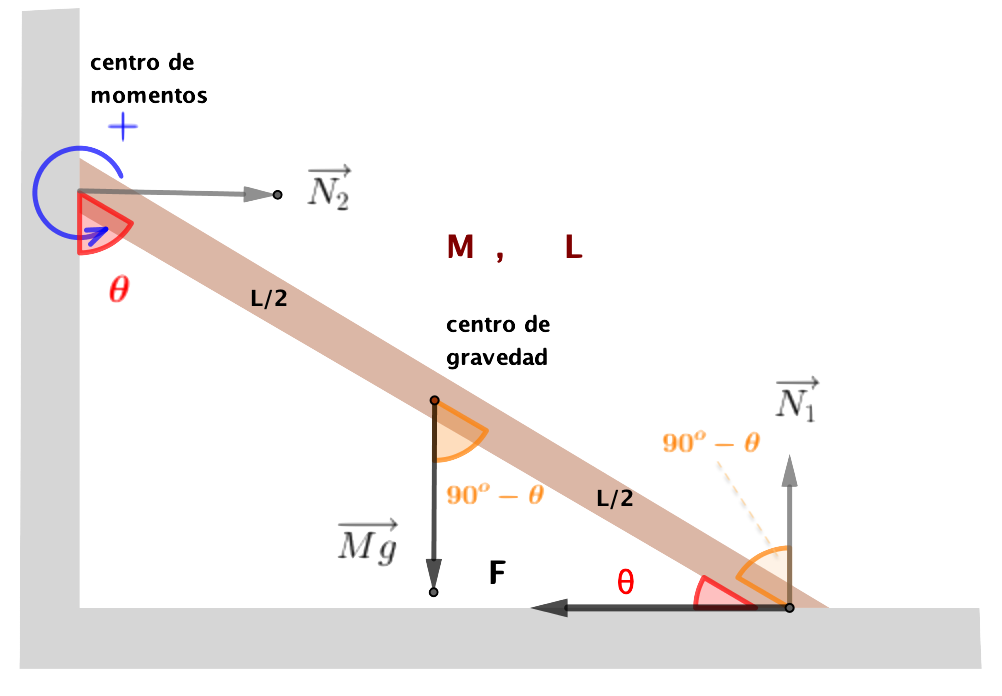
\includegraphics[width=.6\textwidth]{imagenes/img01-02.png}
	\end{figure}
	
\vspace{5mm}

$\boldsymbol{\displaystyle \sum \overrightarrow F = \overrightarrow 0} \ \ \to \ \ \overrightarrow N_2 + \overrightarrow {Mg} + \overrightarrow N_1 + \overrightarrow F = \overrightarrow 0$

Colocando en la esquina el sistema de referencia, 

$(N_2,0) + (0,-Mg)+(0,N_1)+(-F,0) \ \to \ \begin{cases}
\quad N_2-F=0 \\ \ -Mg+N_1=0 	
 \end{cases}
 \ \to \ $
 
 \begin{multicols}{2}
 \begin{equation}
\to \quad \boxed{ \  F = N_2 \ }
	\label{N1}
 \end{equation}
  \begin{equation}
; \qquad \qquad \boxed{ \  N_1 = Mg  \ } \qquad 
	\label{N2}
 \end{equation}
\end{multicols}

\textcolor{gris}{$\overrightarrow M = \overrightarrow F \times \overrightarrow F; \quad M=r\ F\ \sin \alpha$, siendo $\overrightarrow r$ el vector desde el eje (centro) de  momentos al punto de aplicación de cada fuerza $\overrightarrow F$ y  $\alpha$ el ángulo que forman $\overrightarrow r$ y $\overrightarrow F$}

Elegimos, arbitrariamente, el centro de momentos en el punto de aplicación de $\overrightarrow N_2$, punto de contacto de la barra con la pared vertical.

$\boldsymbol{\displaystyle \sum \overrightarrow M = \overrightarrow 0} \ \ \to \ $ 
$\cancelto{0}{N_2 \ 0 \ \sin (90^o-\theta)}-\dfrac L 2 \ Mg \sin (90^o-\theta)- L\ F\ \sin \theta + L \ N_1\ \sin (90^o -\theta)=0$

Despejando: $\ \sin (90^o-\theta)=\cos \theta \ \to \ N_1 \cos \theta = \dfrac 1 2 M g \cos \theta + F \sin \theta$, dividiendo por $\cos \theta$:

\begin{equation}
\boxed{ \ N_1 \ = \ \dfrac 1 2 M g \ + \ F \tan \theta \ }
\label{N3}	
\end{equation}

Nuestros datos eran $\ M, \ L \text{ y } \theta \ $ y nuestras incógnitas $\ N_1,\ N_2, \ \boldsymbol F.\ $ De las ecuaciones \ref{N1},  \ref{N2} y \ref{N3},  obtenemos:

\begin{large}
\begin{equation}
	\subrayado{ \ \boxed{\ \boldsymbol{ F \ = \ \dfrac{Mg}{2\tan \theta}} \ } \ }
\label{R1}	
\end{equation}
\end{large}


	

	

\vspace{0.5cm}
\subsection{Resolución por el principio de \emph{D'Alembert}}
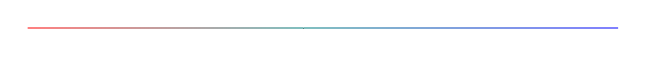
\begin{tikzpicture}
	\fill [left color=red!50, right color=teal!50] (0,0) rectangle (3.5,.01);
	\fill [left color=teal!50, right color=blue!50] (3.5,0) rectangle (7.5,.01);
	\end{tikzpicture}
\vspace{0.5cm}

\begin{myexampleblock}{Desplazamientos virtuales. Principio de D'Alembert}

%\begin{ejemplo}
\begin{small}
Por \emph{desplazamiento virtual} infinitesimal de un sistema físico se entiende una variación de su configuración como resultado de cualquier cambio infinitesimal arbitrario $\ \boldsymbol{\var \vec r_i} \ $ de las coordenadas del sistema compatible con las fuerzas y ligaduras impuestas al mismo en un instante dado $ t $. Es un cambio infinitesimal del sistema de coordenadas que ocurre mientras el tiempo se mantiene fijo. Se le llama \emph{virtual} en vez de real dado que ningún desplazamiento real puede ocurrir sin que el tiempo avance (solo ocurren en nuestra imaginación). La condición de equilibrio es independiente del tiempo real, es como si congelásemos el tiempo.


\vspace{2mm}En la mecánica analítica el concepto de desplazamiento virtual solo es significativo cuando se analiza un sistema físico sujeto a ligaduras que restringen su movimiento. El desplazamiento virtual $\var r$  es un caso especial de desplazamiento infinitesimal (normalmente denotado por $\dd r$) que se refiere a un cambio infinitesimal en las coordenadas de posición de un sistema de manera que las ligaduras se satisfacen.



\begin{destacado}
\textbf{Principio de D'Alembert}. \footnote{Enunciado por Jean Le Rond D'Alembert en 1743, en su obra ``Tratado de la dinámica''.}

\emph{Para que un sistema de puntos materiales esté en equilibrio bajo la acción de un conjunto de fuerzas aplicadas es necesario y suficiente que sea nula la suma de los trabajos virtuales elementales efectuados por estas fuerzas para cualquier desplazamiento virtual de dicho sistema efectuado a partir de una posición de equilibrio.}
\end{destacado}

 
 \begin{equation*}
 \subrayado{\boxed{\ \boldsymbol{\sum_i \vec F_i\cdot \var \vec r_i}=0 \ }}	\qquad \qquad  \text{(ec. \ref{DA})}
 \end{equation*}


El trabajo total efectuado por las fuerzas aplicadas es nulo.

\end{small}
\begin{multicols}{2}
\begin{small}
La figura muestra una aplicación sencilla de este principio a un sistema de una sola partícula y una sola fuerza aplicada, el peso.

El punto $B$ no es un punto de equilibrio, pues en el desplazamiento virtual indicado en la figura el peso realiza trabajo. El punto $A$ si es de equilibrio, pues cualquier desplazamiento virtual es perpendicular al peso y, por tanto, el peso no realiza trabajo. 
\end{small}
\begin{figure}[H]
	\centering
	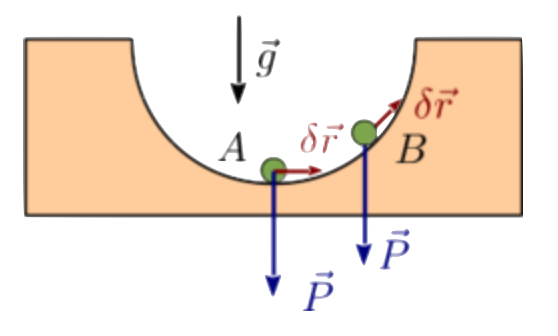
\includegraphics[width=.4\textwidth]{imagenes/img01-03.png}
\end{figure}
\end{multicols}

\begin{flushright}
\rule{200pt}{0.1pt}

\begin{scriptsize}
`Física General', Ignacio Vallés, \textcolor{blue}{http://igvaori.github.io}
\end{scriptsize}
\end{flushright}
%\end{ejemplo}
\end{myexampleblock}

\vspace{0.5cm}
Las condiciones de equilibrio el principio de D'Alembert (estático) es

\vspace{5mm}
\begin{myalertblock}{Principio de D'Alembert: equilibrio estático}

$\,$

\begin{Large}
\begin{equation*}
\sum_i \ \overrightarrow F_i^{(a)} \ \cdot \ \var \overrightarrow r_i \ = \ 0  \qquad \qquad  \text{(ec. \ref{DA})}
\end{equation*}
\end{Large}
	
\end{myalertblock}

\vspace{1cm}
$\overrightarrow N_1 \text{ y } \overrightarrow N_2$ son \emph{fuerzas restrictivas o de ligadura}, son las que no realizan trabajo ante un desplazamiento virtual de la barra, son perpendiculares a ellos. $\overrightarrow{Mg} \text{ y } \overrightarrow F$ son las \emph{fuerzas aplicados o externas}. Aplicando el principio de D'Alambert, tendremos:

\begin{multicols}{2}
$\,$

$\overrightarrow r_1=(L \cos \theta, 0);\quad \overrightarrow r_2= \left( \dfrac L 2 \cos \theta, \dfrac L 2 \sin \theta \right)$

$\displaystyle  \overrightarrow {\var r_1} = \pdv{\overrightarrow r_1}{L} \cancelto{0}{\var L}+ \pdv{\overrightarrow r_1}{\theta} \var \theta = \left( -\dfrac L 2 \sin \theta, \dfrac L 2 \cos \theta \right) \var \theta$

$\displaystyle  \overrightarrow {\var r_2} = \pdv{\overrightarrow r_2}{L} \cancelto{0}{\var L}+ \pdv{\overrightarrow r_2}{\theta} \var \theta = \left( - L  \sin \theta, 0 \right) \var \theta$
\begin{figure}[H]
	\centering
	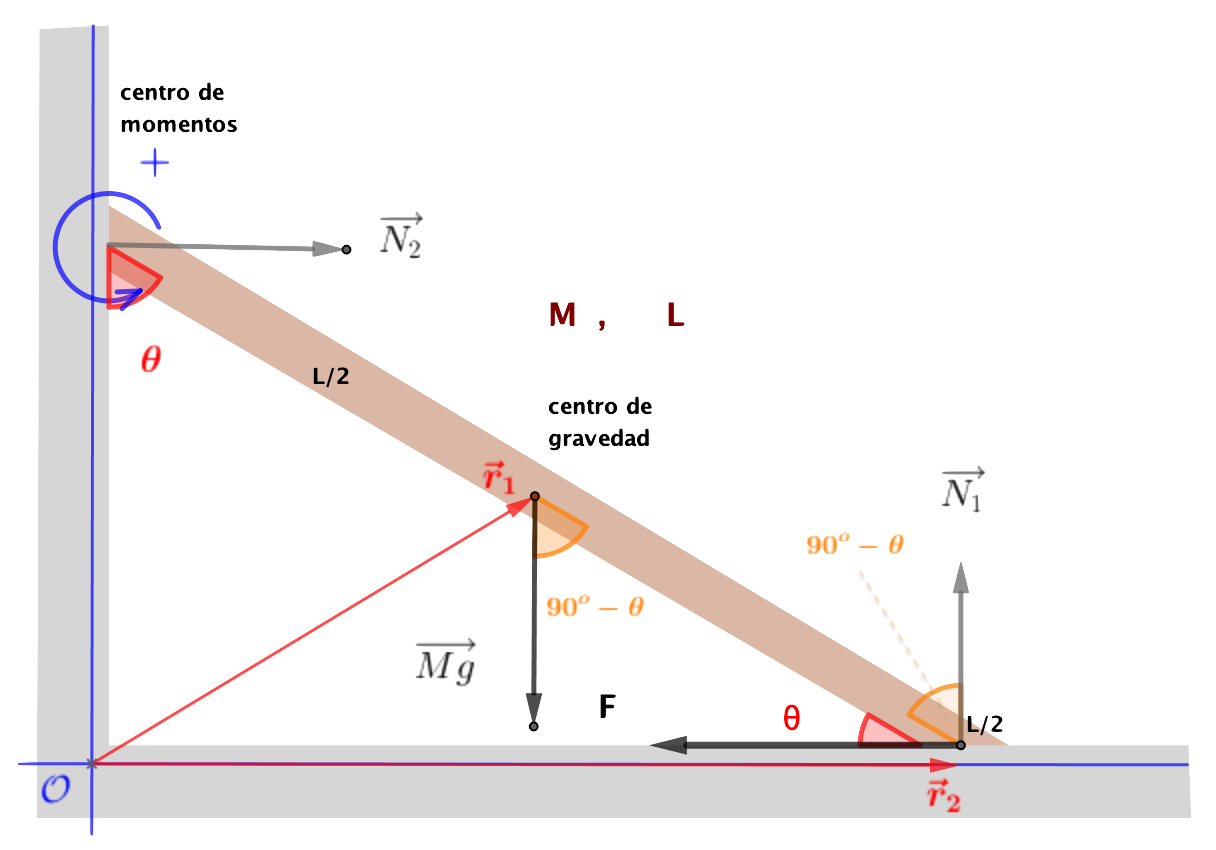
\includegraphics[width=.4\textwidth]{imagenes/img01-04.png}
\end{figure}
\end{multicols}

Ya que la longitud de la barra no varía en un desplazamiento virtual, $\ \var L = 0$, no sería compatible con las ligaduras.

Aplicando el principio de D'Alembert, tendremos:


$\overrightarrow{Mg} \cdot  \overrightarrow {\var r_1} + \overrightarrow F \cdot  \overrightarrow {\var r_2} =(0,-Mg)\cdot \left( -\dfrac L 2 \sin \theta, \dfrac L 2 \cos \theta \right) \var \theta +
(-F,0) \cdot  \left( - L  \sin \theta, 0 \right) \var \theta =0$

$-\dfrac{MgL}2 \cos \theta \ \var \theta + FL\sin \theta \ \var \theta =0$
$\ \to \ $
$\cancelto{\neq 0}{L} \ \left[ -\dfrac{Mg}{2} \cos \theta+ F \sin \theta \right] \ \cancelto{\neq 0}{\var \theta }= 0$

La barra tiene una determinada longitud no nula ($\cancelto{\neq 0}{L}$) y, por hipótesis, estamos considerando un desplazamiento virtual no nulo ($\cancelto{\neq 0}{\var \theta}$). Despejando, obtenemos el mismo resultado que aplicando la mecánica newtoniana:

\begin{large}
\begin{equation}
	\subrayado{ \ \boxed{\ \boldsymbol{ F \ = \ \dfrac{Mg}{2\tan \theta}} \ } \ }
\label{R1}	
\end{equation}
\end{large}






